% !TeX root = main.tex

% ============================================================
% thesis-sync entry: 2026-07-19_inchworm-bending-experiment
% Type: experimental result (bending angle vs pressure)
% Part of the INCHWORM ROBOT block (prior work, precedes the lizard sections).
% Insertable section block (no preamble). Requires: graphicx.
% ============================================================

\section{ACTUATOR BENDING CHARACTERIZATION}
\label{sec:inchworm-bending-experiment}

To evaluate the bending performance of the fabricated actuator, an
experimental setup was developed. A diagram of the setup and the
experiment's results are shown in Fig.~\ref{fig:inchworm-experiment}. The
actuator was suspended vertically and secured by a clamp at its tip. A
manually operated syringe was connected to one of the actuator's chambers,
in-line with a pressure sensor. The bending deformation was recorded using a
camera, and the resulting video was analyzed using ImageJ software to
extract the bending angle via optical measurement. Working against gravity,
the actuator achieved a bending angle of $180^\circ$ at a pressure of
approximately 15.5~kPa when a single chamber was pressurized.

\begin{figure}[tb]
 \centering
  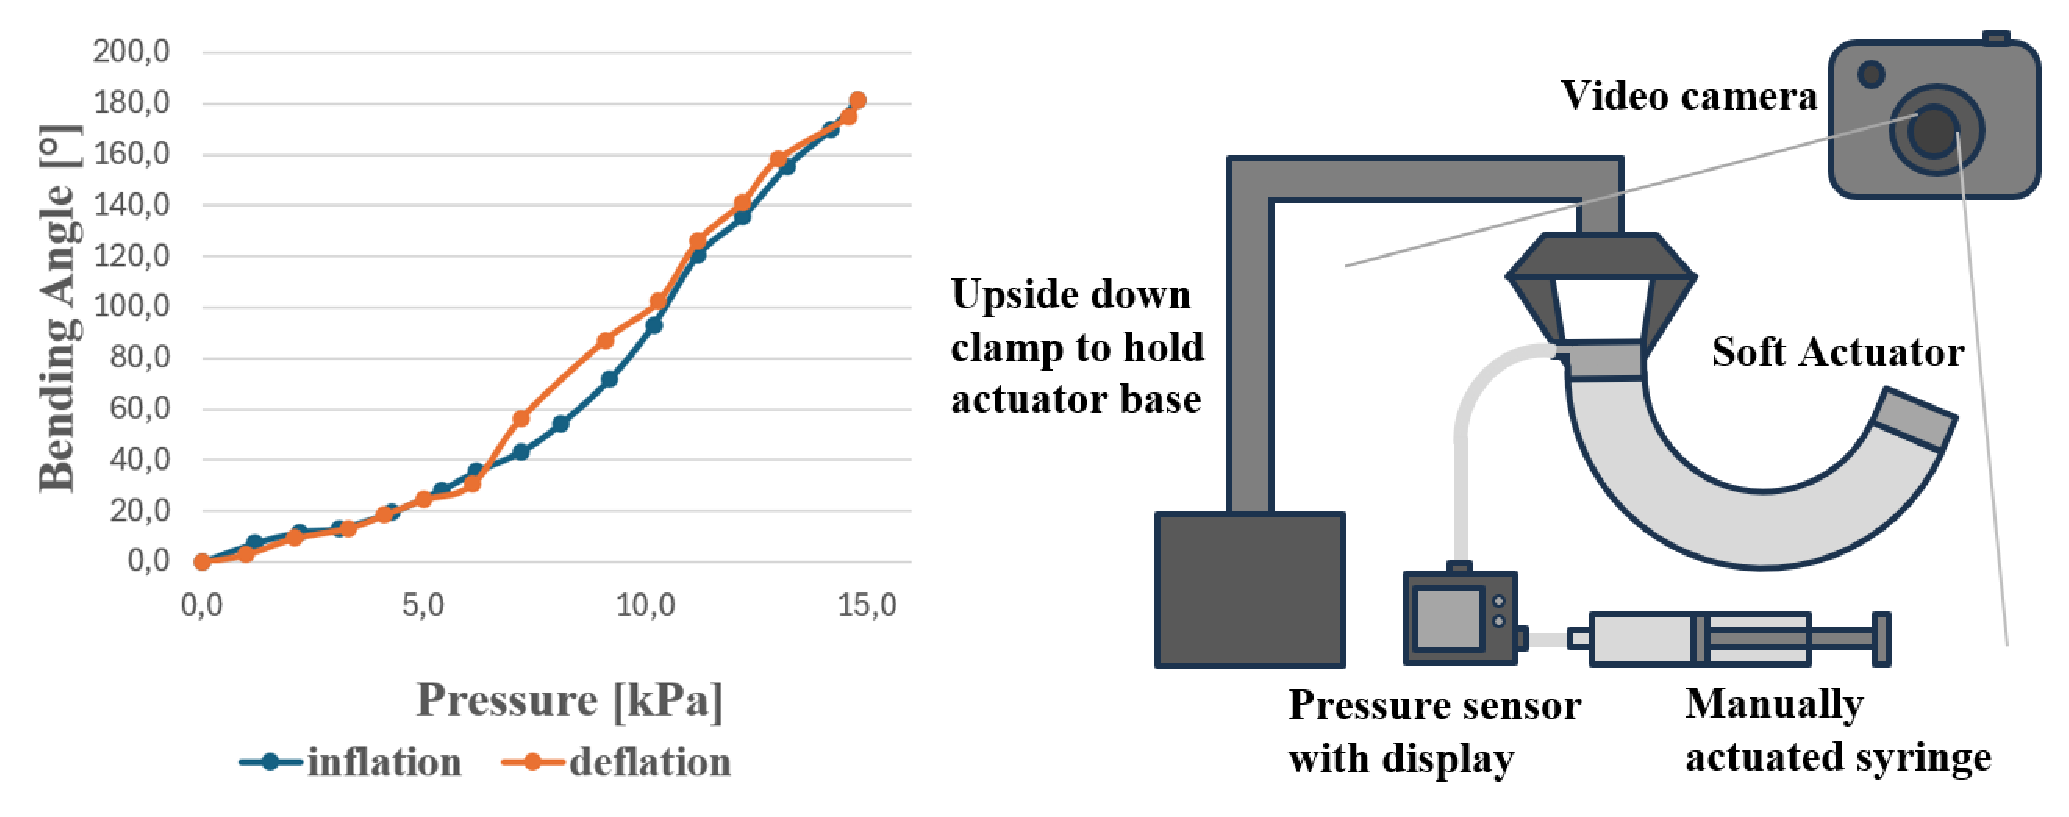
\includegraphics[height=34mm]{figures/experiment.eps}
  \vspace*{-4mm}
  \caption{Evaluation of the soft actuator. (Left) Bending angle versus
  applied pressure when pressurizing a single chamber. (Right) Experimental
  setup.}
  \label{fig:inchworm-experiment}
\end{figure}
